\begin{frame}
\frametitle{Rectangular/Cartesian Coordinates}

\begin{itemize}
\item To reach the projector: \pause Must relate its position to
\begin{itemize}
\item My current position
\item My current orientation
\end{itemize}

\item<3-> Rectangular Coordinate System
\begin{itemize}
\item Position $\to$ Origin $\to$ $O$;
\item Orientation $\to$ Fundamental directions $\to$ Ahead-Left-Up;
\item Displacement $\to$ measured using the distance:
\begin{itemize}
\item Positive in Ahead, Left, and Up directions;
\item Negative in Back, Right, and Down directions.
\end{itemize}
\end{itemize}

\item<4-> Example: Projector $P \to (x,y,z) = (3,1,2)$ or $P(3,1,2)$.

\item<5-> Using a fixed coordinate system:
\begin{itemize}
\item $\text{Space } \simeq \RR \times \RR \times \RR = \RR^3$
\item $\text{Plane } \simeq \RR \times \RR = \RR^2$
\end{itemize}
\end{itemize}
\end{frame}

\begin{frame}
%
\begin{table}[h]
\begin{tabular}{lcr}
\psfrag{P}{Projector}
\psfrag{O}{Me}  
\psfrag{x}{$x$} 
\psfrag{y}{$y$} 
\psfrag{z}{$z$}     
\psfrag{A}{Ahead}
\psfrag{L}{Left}
\psfrag{U}{Up}  
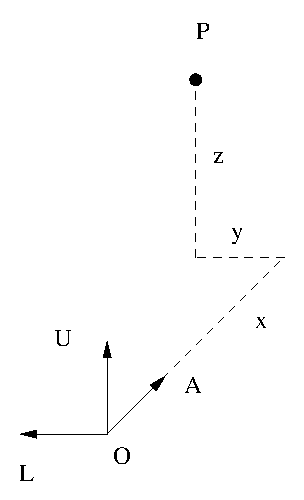
\includegraphics[height=2in]{../../modules/coordinate-systems/pictures/projector.eps}
%
& \hspace{2cm} &
%
%\begin{figure}[h]
\psfrag{P}{$P(a,b,c)$}
\psfrag{O}{$O(0,0,0)$}  
\psfrag{x}{$a$} 
\psfrag{y}{$b$} 
\psfrag{z}{$c$}     
\psfrag{A}{$Ox$}
\psfrag{L}{$Oy$}
\psfrag{U}{$Oz$}  
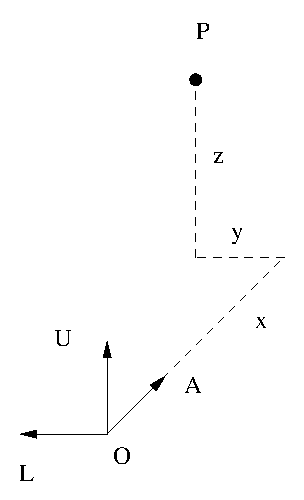
\includegraphics[height=2in]{../../modules/coordinate-systems/pictures/projector.eps}
%
\end{tabular}
\end{table}
%
\end{frame}